\documentclass[12pt, a4paper]{article}

\usepackage[T1]{fontenc}
\usepackage{graphicx}
\usepackage{hyperref}
\usepackage[brazil]{babel}
\usepackage{geometry}
\usepackage{color}
\usepackage{pythonhighlight}
\usepackage[utf8]{inputenc}
\usepackage{indentfirst}
\usepackage{verbatim}
\usepackage{multirow}
\usepackage{booktabs}

\lstset{
	numbers=left,
}

\geometry{
	a4paper,
	left=30mm,
	right=20mm,
	top=30mm,
	bottom=20mm
}

\title{
    \textbf{IESB} \\
    \large Big Data e Inteligência Analítica \\
    \vspace{10cm}
    \textbf{Projeto Integrador em Big Data e Inteligência Analítica}
    \author{Lucas Siqueira Rodrigues}
    \date{}
}

\begin{document}

\begin{titlepage} 
    \maketitle
    \begin{center}
        \vspace{\fill}
        Brasília - DF \\
        Junho de 2025
    \end{center}
\end{titlepage}

\section{Obtenção da base de dados}
\subsection{Introdução}
O trabalho tem como objetivo explorar os dados públicos disponibilizados pela Câmara dos Deputados para analisar e compreender os gastos realizados pelos parlamentares. Para isso, os dados serão obtidos por meio do portal dos dados abertos da câmara\cite{dados_abertos}, armazenados em um banco de dados relacional na nuvem e, posteriormente, analisados.

\subsection{Motivação}
A transparência pública é essencial para garantir a confiança da população nas instituições governamentais. Esse projeto busca realizar um ciclo completo de extração, transformação, armazenamento e análise dos dados de gastos públicos. Além disso, ao construir dashboards dinâmicos espera-se fornecer ferramentas que possam auxiliar na identificação de possíveis irregularidades e na fiscalização das despesas parlamentares.


\subsection{Script e Banco de Dados}
Para o ano de 2022, a obtenção dos dados por meio da API\cite{dados_abertos} retornou apenas 32 registros.

\begin{python}
import io
import json
import zipfile

import httpx
from tqdm import tqdm

class CamaraAPI:
	def __init__(self) -> None:
		self.base_url = "https://dadosabertos.camara.leg.br/api/v2"
	
	def request(self, endpoint: str) -> dict:
		response = httpx.get(f"{self.base_url}/{endpoint}")
		return response.json()
	
	def get_deputados(self) -> dict:
		return self.request("deputados").get("dados", {})
	
	def get_despesas(self, id_: int, year: int = 2022) -> dict:
		return self.request(f"deputados/{id_}/despesas?ano={year}")

despesas = []

api = CamaraAPI()

deputados = api.get_deputados()
for deputado in tqdm(deputados):
	id_ = deputado["id"]
	despesas_deputado = api.get_despesas(id_=id_, year=2022)
	despesas.extend(despesas_deputado["dados"])

print(len(despesas))  # output: 32
\end{python}

Por isso, apenas para esse ano a coleta de dados foi por meio de um arquivo no formato JSON, que também é fornecido no portal de dados abertos da câmara por meio da aba “Arquivos”.

\begin{figure}[!htbp]
    \centering
    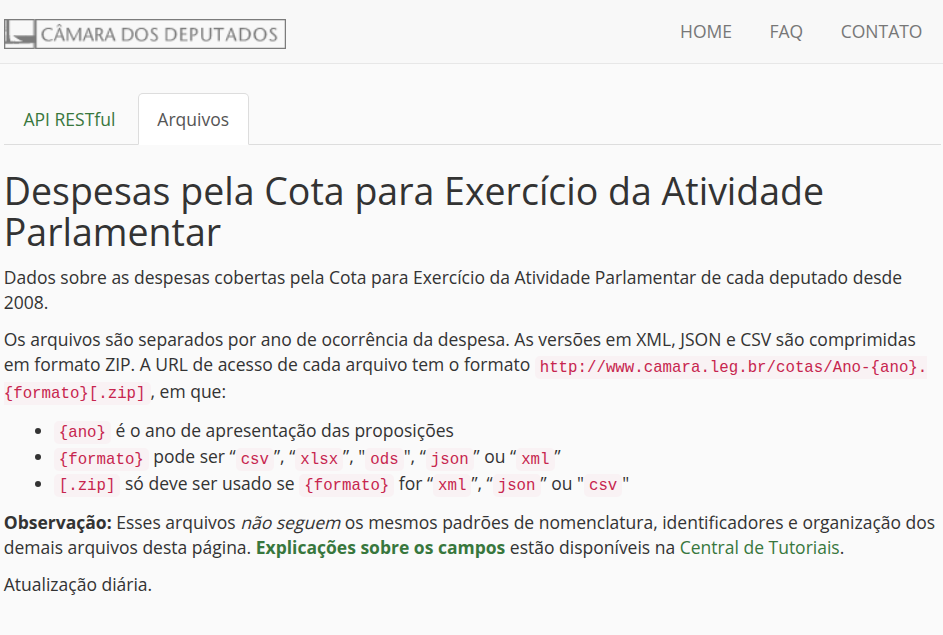
\includegraphics[width=0.8\textwidth]{assets/1_arquivos.png}
    \caption{Coleta de dados por meio da aba de arquivos.}
    \label{fig:arquivo_json}
\end{figure}

Para os anos de 2023 e 2024 a obtenção dos dados foi realizada por meio da API\cite{dados_abertos} da Câmara dos Deputados, explorando dois principais endpoints:
\begin{itemize}
    \item \texttt{/deputados}: Retorna informações gerais sobre os parlamentares, como seus nomes, partidos, estados e e-mails.
    \item \texttt{/deputados/\{id\}/despesas}: Fornece detalhes sobre as despesas realizadas pelos parlamentares, incluindo valores, fornecedores, tipos de despesa e datas.
\end{itemize}

Para organizar os dados de forma eficiente e integrar os dados obtidos por meio da API e por meio do JSON, foi criado um modelo de banco de dados relacional com tabelas normalizadas para representar as informações de deputados, despesas e fornecedores\cite{dbdiagram}.

\begin{figure}[!htbp]
	\centering
	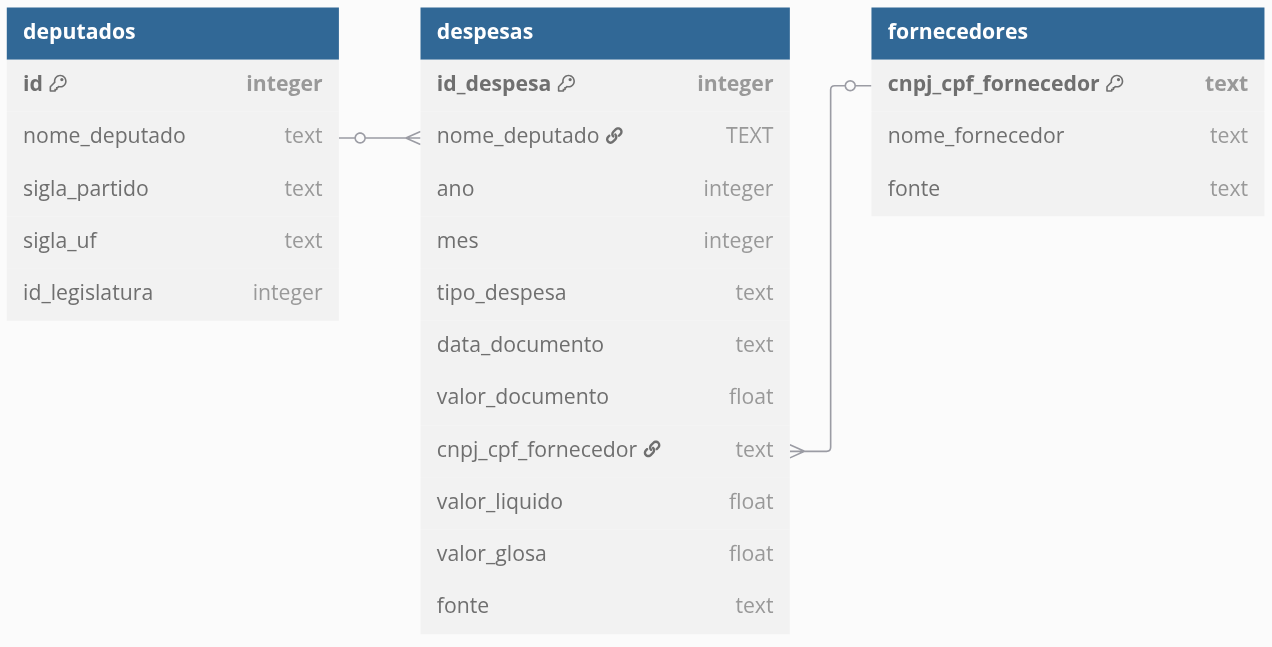
\includegraphics[width=0.8\textwidth]{assets/1_dbdiagram.png}
	\caption{Diagrama relacional.}
	\label{fig:arquivo_json}
\end{figure}

Os dados são obtidos e unificados por meio da classe DataService.

\begin{python}
import io
import json
import re
import zipfile

import httpx
from tqdm import tqdm

from data_ingestion.services.log_service import logger


class DataService:
	def __init__(self) -> None:
	self.api_base_url = "https://dadosabertos.camara.leg.br/api/v2"
	
	def get_deputados(self) -> list:
		response = httpx.get(f"{self.api_base_url}/deputados")
		data = response.json().get("dados")
		selected_data = [
			{
				"id": i["id"],
				"nome": i["nome"],
				"sigla_partido": i["siglaPartido"],
				"id_legislatura": i["idLegislatura"],
				"sigla_uf": i["siglaUf"],
			}
			for i in data
			]
	
		return selected_data
	
	def get_data_from_api(self, anos: list[int]) -> tuple[list[dict], list[dict], list[dict]]:
		deputados = self.get_deputados()
		despesas = []
		fornecedores = []
		for ano in anos:
			logger.info(f"Getting data from API for year {ano}")
			for deputado in tqdm(deputados):
				response = httpx.get(f"{self.api_base_url}/deputados/{deputado['id']}/despesas?ano={ano}")
				despesas_deputado = response.json().get("dados")
		
				for item in despesas_deputado:
					despesas.append({
						"nome_deputado": deputado.get("nome"),
						"ano": item.get("ano"),
						"mes": item.get("mes"),
						"tipo_despesa": item.get("tipoDespesa"),
						"data_documento": item.get("dataDocumento"),
						"valor_documento": item.get("valorDocumento"),
						"cnpj_cpf_fornecedor": re.sub(r"[^0-9]", "", item.get("cnpjCpfFornecedor")),
						"valor_liquido": item.get("valorLiquido"),
						"valor_glosa": item.get("valorGlosa"),
						"fonte": "api",
					})
		
					fornecedores.append({
						"nome_fornecedor": item.get("nomeFornecedor"),
						"cnpj_cpf_fornecedor": re.sub(r"[^0-9]", "", item.get("cnpjCpfFornecedor")),
						"fonte": "api",
					})
		
		logger.info(f"Total number of despesas: {len(despesas)}")
		
		return deputados, despesas, fornecedores
	
	@staticmethod
	def get_data_from_url(url: str) -> tuple[list[dict], list[dict], list[dict]]:
		logger.info(f"Getting data from url: {url}")
		response = httpx.get(url=url)
		zip_content = response.content
		
		with zipfile.ZipFile(io.BytesIO(zip_content)) as zip_file:
			with zip_file.open(zip_file.namelist()[0]) as json_file:
				json_content = json_file.read().decode("utf-8")
				json_data = json.loads(json_content).get("dados")
		
		deputados = []
		despesas = []
		fornecedores = []
		
		for item in json_data:
			deputados.append({
				"id": item["numeroDeputadoID"],
				"nome": item["nomeParlamentar"],
				"sigla_partido": item["siglaPartido"],
				"id_legislatura": item["codigoLegislatura"],
				"sigla_uf": item["siglaUF"],
			})
			
			despesas.append({
				"nome_deputado": item.get("nomeParlamentar"),
				"ano": item.get("ano"),
				"mes": item.get("mes"),
				"tipo_despesa": item.get("descricao"),
				"data_documento": item.get("dataEmissao"),
				"valor_documento": item.get("valorDocumento"),
				"cnpj_cpf_fornecedor": re.sub(r"[^0-9]", "", item.get("cnpjCPF")),
				"valor_liquido": item.get("valorLiquido"),
				"valor_glosa": item.get("valorGlosa"),
				"fonte": "url",
			})
			
			fornecedores.append({
				"nome_fornecedor": item.get("fornecedor"),
				"cnpj_cpf_fornecedor": re.sub(r"[^0-9]", "", item.get("cnpjCPF")),
				"fonte": "url",
			})
		
		logger.info(f"Total number of despesas: {len(despesas)}")
		
		return deputados, despesas, fornecedores
\end{python}


Por fim, temos a função main(), que realiza todo o ciclo de extração, transformação e carregamento dos dados.

\begin{python}
import os

from dotenv import load_dotenv

from data_ingestion.services.data_service import DataService
from data_ingestion.services.db_service import DBService

_ = load_dotenv()


def main() -> None:
	url = "https://www.camara.leg.br/cotas/Ano-2022.json.zip"
	anos = [2023, 2024]
	
	data_service = DataService()
	api_deputados, api_despesas, api_fornecedores = data_service.get_data_from_api(anos=anos)
	url_deputados, url_despesas, url_fornecedores = data_service.get_data_from_url(url=url)
	
	deputados = [*api_deputados, *url_deputados]
	despesas = [*api_despesas, *url_despesas]
	fornecedores = [*api_fornecedores, *url_fornecedores]
	
	db_service = DBService(
		user=os.environ["DB_USER"],
		password=os.environ["DB_PASSWORD"],
		host=os.environ["DB_HOST"],
		port=int(os.environ["DB_PORT"]),
		dbname=os.environ["DB_NAME"],
	)
	db_service.insert_data(deputados=deputados, despesas=despesas, fornecedores=fornecedores)


if __name__ == "__main__":
	main()
\end{python}

O programa, ao ser executado, faz a extração, transformação e carga de 223.982 registros de despesas dos anos de 2022, 2023 e 2024.

Logo após serem obtidos, os dados foram inseridos em um banco de dados MySQL, que foi criado usando o serviço Amazon RDS (Relational Database Service).

\begin{figure}[!htbp]
    \centering
    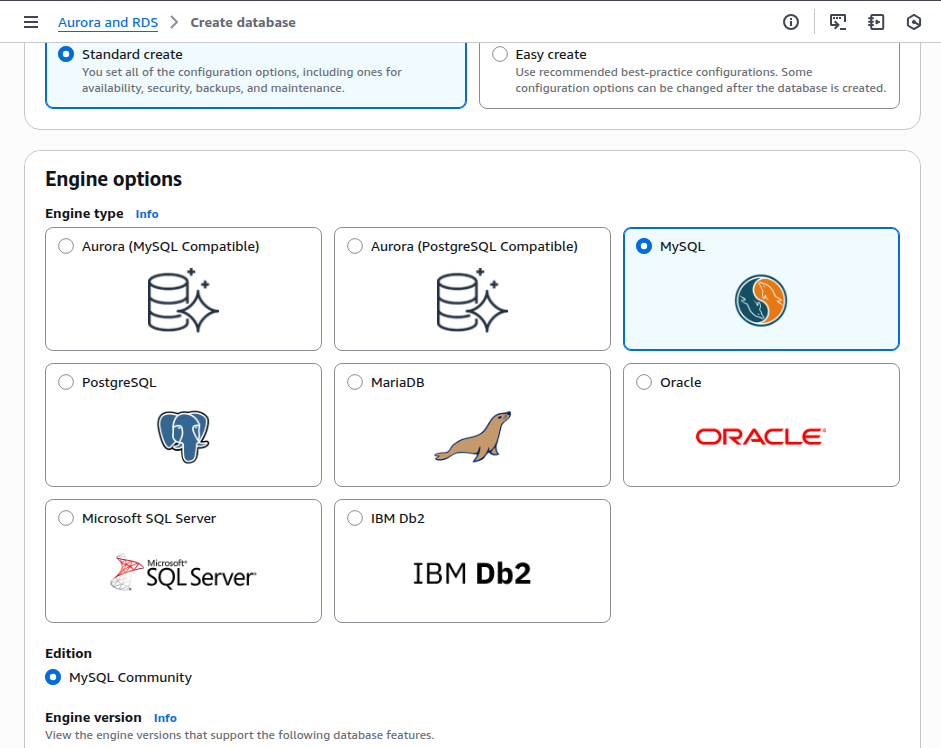
\includegraphics[width=0.8\textwidth]{assets/1_criacao.png}
    \caption{Criação do MySQL na AWS.}
    \label{fig:criacao_mysql}
\end{figure}

Após a base de dados ser criada, podemos nos conectar a ela usando o DBeaver\cite{dbeaver}.

\begin{figure}[!htbp]
    \centering
    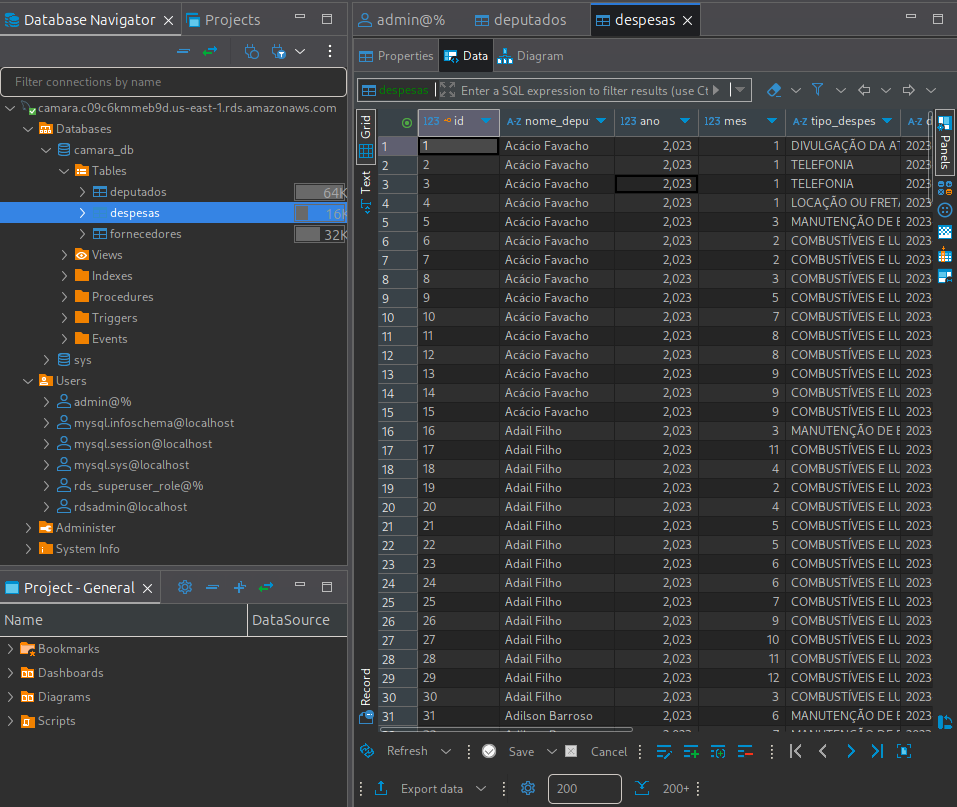
\includegraphics[width=0.8\textwidth]{assets/1_dbeaver.png}
    \caption{Base de dados conectada no DBeaver.}
    \label{fig:db conexão}
\end{figure}

Todo o código relacionado ao projeto está no Github\cite{github_repo}.

\subsection{Considerações finais}

A combinação de tecnologias como Python, AWS e MySQL foi fundamental para realizar as etapas de extração, transformação e carregamento dos dados. A API da Câmara revelou-se limitada em relação à quantidade de dados retornados para o ano de 2022, mas a extração dos dados do JSON da aba Arquivos permitiu superar essa restrição e criar uma base robusta com uma quantidade considerável de dados.

\section{Relatório Analítico}

\subsection{Introdução}

A análise de dados públicos desempenha um papel crucial na promoção da transparência governamental e no combate a irregularidades. Utilizando o Streamlit para a criação de dashboards, é possível transformar grandes volumes de dados em informações compreensíveis e acessíveis para a população e órgãos de fiscalização.

\subsection{Demonstração}

O Streamlit foi integrado ao banco de dados MySQL, permitindo consultas em tempo real e construção de dashboards dinâmicos.

Na nossa base de dados foram construídas 3 tabelas, e para facilitar o processo de construção de gráficos uma query foi feita realizando o join das tabelas.

\begin{verbatim}
SELECT
	despesas.nome_deputado,
	despesas.ano,
	despesas.mes,
	despesas.tipo_despesa,
	despesas.valor_documento,
	despesas.cnpj_cpf_fornecedor,
	deputados.sigla_partido,
	deputados.id_legislatura,
	deputados.sigla_uf,
	fornecedores.nome_fornecedor
FROM
	despesas
LEFT JOIN
	deputados on despesas.nome_deputado = deputados.nome
LEFT JOIN
	fornecedores ON despesas.cnpj_cpf_fornecedor = fornecedores.cnpj_cpf_fornecedor;
\end{verbatim}

A partir dos dados recuperados da base de dados criamos um dataframe do Pandas\cite{Pandas}, onde podemos aplicar filtros e realizar agrupamentos nos dados para extrair informações e criar gráficos.

\begin{python}
grouped_df = df[["tipo_despesa", "valor_documento"]].groupby("tipo_despesa").sum()
st.bar_chart(grouped_df, horizontal=True, x_label="Valor total em R$")
\end{python}

\begin{figure}[!htbp]
	\centering
	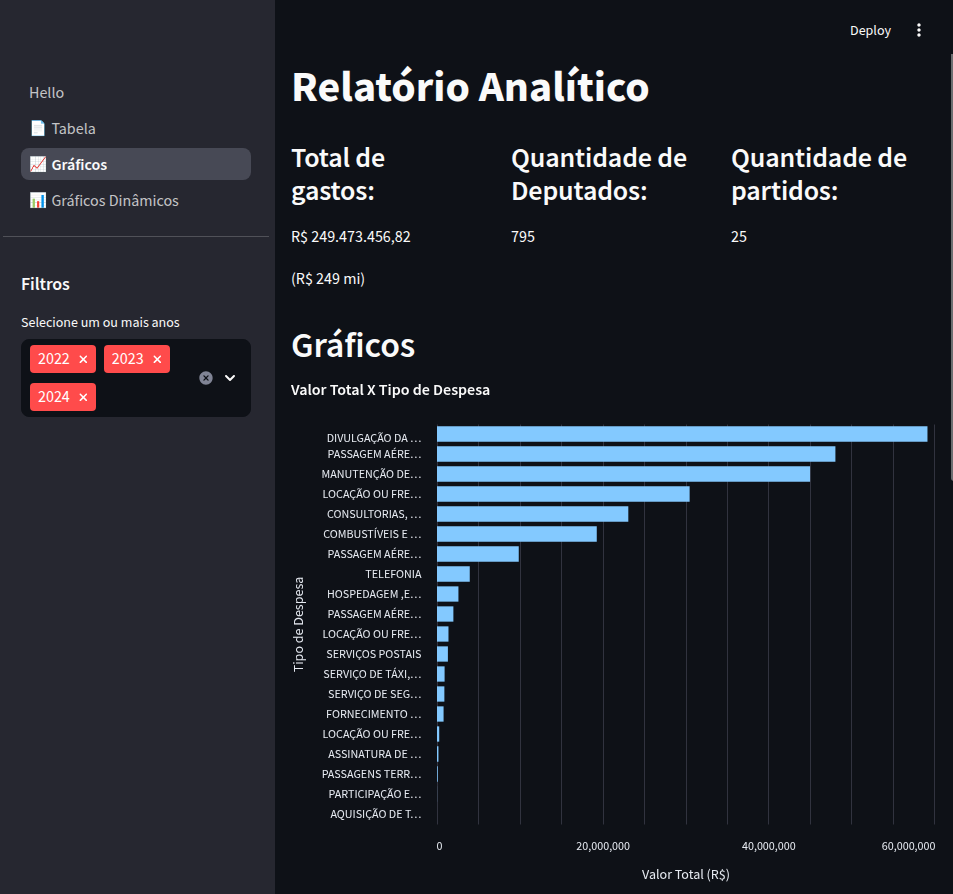
\includegraphics[width=0.8\textwidth]{assets/2_plot1.png}
	\caption{Gráfico mostrando a quantidade de gastos por tipo de despesa.}
	\label{fig:criacao_postgresql}
\end{figure}

\subsection{Relatórios e tabelas}

Aqui podemos analisar o gastos dos anos de 2022, 2023 e 2024 de forma combinada ou isolada. Temos que o total de gastos são:

\begin{table}[htbp]
	\centering
	\begin{tabular}{llll}
		\toprule
		Ano & Total de Gastos & Quantidade de Deputados \\
		\midrule
		Combinados & R\$ 249 mi & 795 \\
		2022 & R\$ 221 mi & 572 \\
		2023 & R\$ 14 mi & 494 \\
		2024 & R\$ 14 mi & 496 \\
		\bottomrule
	\end{tabular}
	\caption{Resumo de gastos.}
	\label{tab:minhatabela1}
\end{table}

Para os anos combinados, temos que DIVULGAÇÃO DA ATIVIDADE PARLAMENTAR foi a categoria de gastos com o maior valor, seguido de PASSAGEM AÉREA - SIGEPA e MANUTENÇÃO DE ESCRITÓRIO DE APOIO À ATIVIDADE PARLAMENTAR.

\begin{figure}[!htbp]
	\centering
	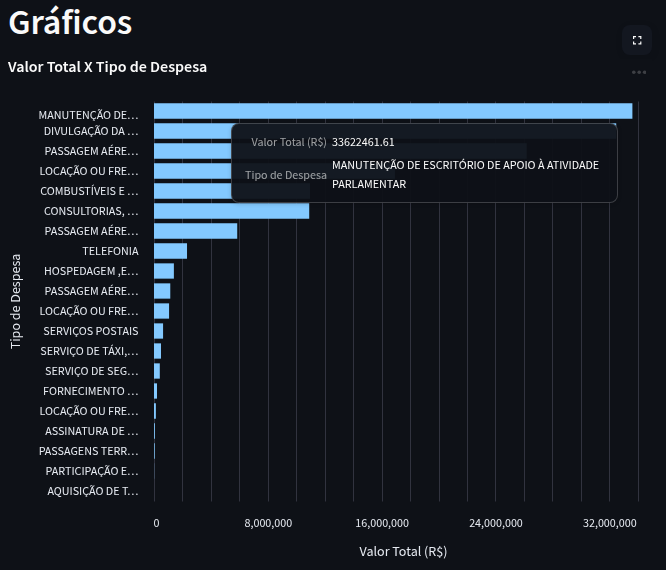
\includegraphics[width=0.8\textwidth]{assets/2_plot2.png}
	\caption{Valor dos gastos por tipo de despesa.}
	\label{fig:criacao_postgresql}
\end{figure}

Giacobo foi o parlamentar com a maior quantidade de gastos, totalizando R\$ 1.289.809,76 em gastos, seguido por Silas Câmara com R\$ 1.177.321,09 e Gustinho Ribeiro com R\$ 1.061.509,11.

\begin{figure}[!htbp]
	\centering
	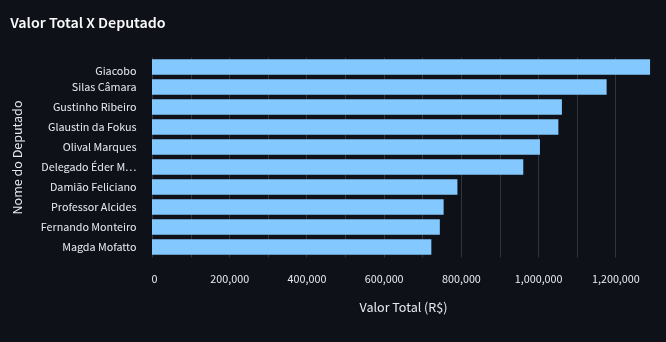
\includegraphics[width=0.8\textwidth]{assets/2_plot3.png}
	\caption{Valor dos gastos por deputado.}
	\label{fig:criacao_postgresql}
\end{figure}

Com relação aos fornecedores, as 3 maiores são empresas de companhias aéreas. A TAM foi disparadamente a maior, com gastos totalizando R\$ 48 milhões, seguida por Latam Linhas Aéreas com R\$ 5 milhões e Gol Linhas Aéreas com quase R\$ 4 milhões.

\begin{figure}[!htbp]
	\centering
	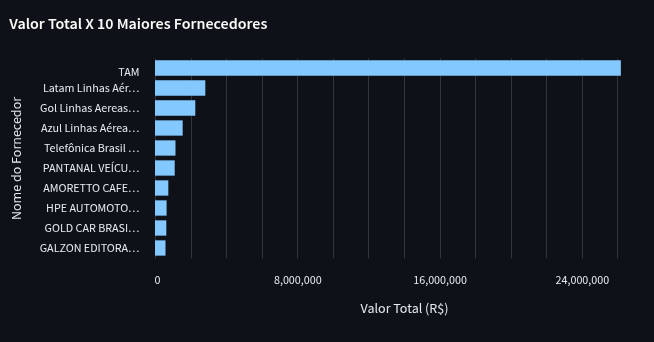
\includegraphics[width=0.8\textwidth]{assets/2_plot4.png}
	\caption{Valor dos gastos por fornecedor.}
	\label{fig:criacao_postgresql}
\end{figure}

Usando o streamlit também podemos criar gráficos dinâmicos para analisar os dados separados por categorias, assim podemos selecionar a variável de interesse e a função de agregação, para assim poder analisar o total de gastos, média, valor máximo e muito mais.

\begin{figure}[!htbp]
	\centering
	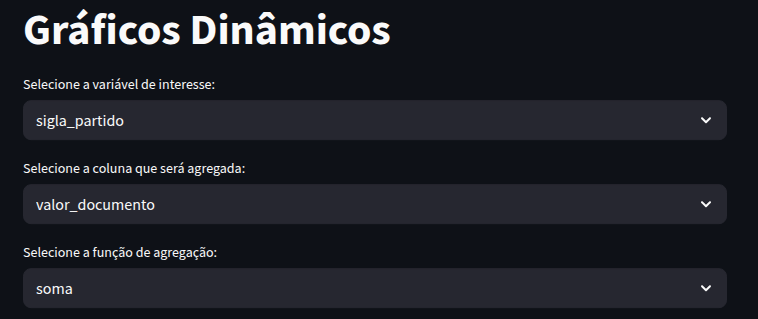
\includegraphics[width=0.8\textwidth]{assets/2_plot5.png}
	\caption{Gráfico dinâmico.}
	\label{fig:criacao_postgresql}
\end{figure}

Ao selecionar a categoria sigla\_partido, podemos ver que os partidos com o maior número de gastos foi o PL com R\$ 34 milhões, seguido pelo PP com R\$ 28 milhões e o PT com R\$ 27 milhões.

\begin{figure}[!htbp]
	\centering
	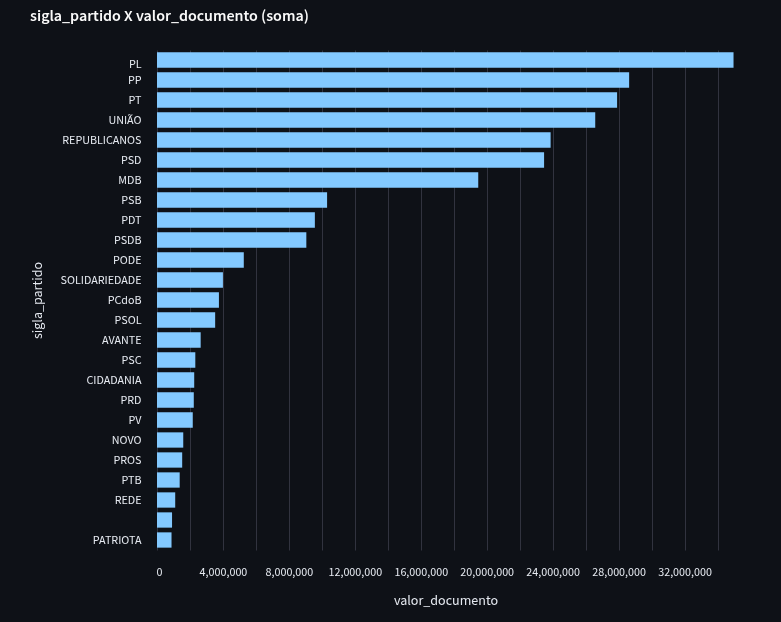
\includegraphics[width=0.8\textwidth]{assets/2_plot6.png}
	\caption{Valor dos gastos por partido.}
	\label{fig:criacao_postgresql}
\end{figure}

\subsection{Considerações finais}

O Streamlit é uma ferramenta robusta para análise de dados, permitindo a criação de gráficos interativos que facilitam a compreensão e a extração de insights valiosos. Diferente de plataformas de BI como o Power BI, o Streamlit oferece maior controle e personalização sobre suas visualizações, embora exija conhecimento em programação e um tempo de desenvolvimento inicial maior.

Uma das suas maiores vantagens é a capacidade de construir gráficos que retornam dados diretamente do banco de dados. Isso garante que suas visualizações estejam sempre atualizadas e em tempo real, proporcionando uma visão dinâmica e precisa das informações.

\section{Machine Learning}
\subsection{Introdução}

Machine Learning (Aprendizado de Máquina) é um campo da inteligência artificial que permite aos sistemas aprender com dados, identificar padrões, tomar decisões e fazer predições futuras com mínima intervenção humana. Sua aplicação vai desde a detecção de anomalias e o reconhecimento de padrões em grandes volumes de dados até a otimização de processos e a personalização de experiências. É uma ferramenta poderosa para transformar dados brutos em insights acionáveis.

\subsection{Dicionário de dados}

No contexto do nosso projeto, as seguintes variáveis são selecionadas para a construção do modelo de machine learning:

\begin{itemize}
	\item \texttt{nome\_deputado}: Retorna o nome completo do deputado.
	\item \texttt{ano}: Indica o ano em que a despesa foi realizada.
	\item \texttt{mes}: Indica o mês em que a despesa foi realizada.
	\item \texttt{tipo\_despesa}: Descreve a categoria da despesa, como "DIVULGAÇÃO DA ATIVIDADE PARLAMENTAR"\ ou  "PASSAGEM AÉREA - SIGEPA".
	\item \texttt{valor\_documento}: Apresenta o valor da despesa conforme registrado no documento fiscal.
	\item \texttt{cnpj\_cpf\_fornecedor}: Fornece o CNPJ ou CPF do fornecedor do bem ou serviço.
	\item \texttt{sigla\_partido}: Retorna a sigla do partido político ao qual o deputado é filiado.
	\item \texttt{id\_legislatura}: Identificador único da legislatura à qual o deputado pertence.
	\item \texttt{sigla\_uf}: Retorna a sigla da Unidade Federativa (estado) pela qual o deputado foi eleito.
	\item \texttt{nome\_fornecedor}: Apresenta o nome completo do fornecedor do bem ou serviço.
\end{itemize}

Com o propósito de criar um modelo de identificação de anomalias nos dados, utilizamos o algoritmo Isolation Forest.

O Isolation Forest é um algoritmo de Machine Learning não supervisionado, amplamente utilizado para detecção de anomalias. Diferente de outros métodos que tentam "encontrar" a normalidade para depois identificar o que é diferente, o Isolation Forest adota uma abordagem mais direta: ele isola as anomalias. Ele funciona da seguinte forma:

\begin{enumerate}
	\item \texttt{Construção de Árvores Aleatórias}: O algoritmo constrói uma floresta de árvores de decisão. Para cada árvore, ele seleciona aleatoriamente um atributo e, em seguida, seleciona aleatoriamente um ponto de divisão dentro do intervalo de valores desse atributo.
	\item \texttt{Isolamento de Pontos}: Esse processo de divisão continua até que cada ponto de dado esteja isolado ou um limite de profundidade da árvore seja atingido.
	\item \texttt{Identificação de Anomalias}: O princípio é que as anomalias, por serem pontos mais raros e diferentes, geralmente exigem menos divisões para serem isoladas nas árvores. Pontos normais, por outro lado, são mais densos e requerem mais divisões para serem separados uns dos outros.
\end{enumerate}

Vantagens do Isolation Forest:

\begin{itemize}
	\item Eficiência: É computacionalmente mais eficiente do que muitos outros algoritmos de detecção de anomalias, especialmente para grandes conjuntos de dados.
	\item Escalabilidade: Lida bem com dados de alta dimensão.
	\item Baixo Consumo de Memória: Não exige o armazenamento de modelos de densidade complexos.
	\item Não Supervisionado: Não requer dados previamente rotulados como "normal" ou "anômalo" para treinar o modelo.
\end{itemize}

Podemos transformar os dados em um dataframe do Pandas\cite{Pandas}, e usá-lo para criar um modelo usando a classe IsolatioForest presente no Scikit-Learn\cite{Scikit-Learn}.

\begin{python}
from sklearn.ensemble import IsolationForest	

df_clean = df.dropna(subset=["valor_liquido"])

X = df_clean[["valor_liquido"]]

iso_forest = IsolationForest(contamination=0.01, random_state=42)
df_clean["anomaly"] = iso_forest.fit_predict(X)

# -1 para anomalias, 1 para dados normais
anomalies = df_clean[df_clean["anomaly"] == -1]
print(f"Temos {len(anomalies)} anomalias no dataframe contendo {len(df)} registros")
print(f"Isso representa {100 * (len(anomalies) / len(df))}% dos registros")

# Temos 2210 anomalias no dataframe contendo 223982 registros
# Isso representa 0.9866864301595665% dos registros
\end{python}

Aqui temos alguns exemplos de dados classificados como anomalias.

\begin{figure}[!htbp]
	\centering
	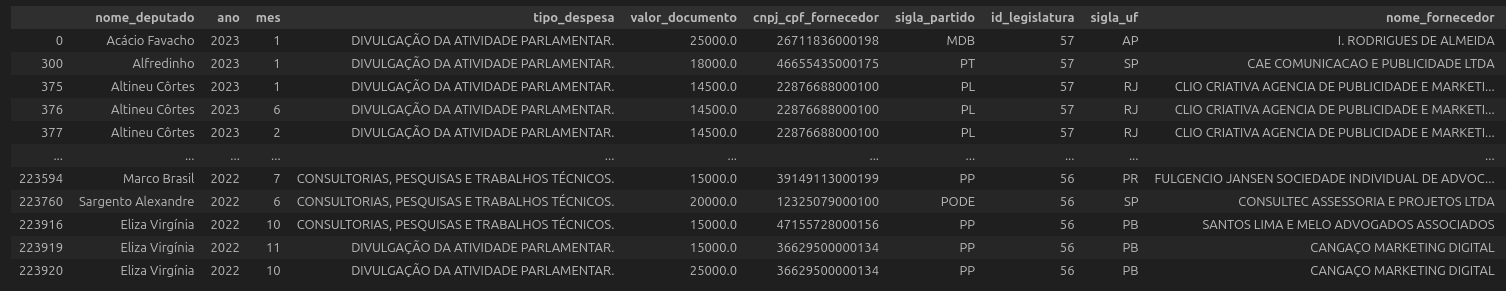
\includegraphics[width=0.8\textwidth]{assets/3_plot1.png}
	\caption{Anomalias nos gastos.}
	\label{fig:anomalias}
\end{figure}

\subsection{Considerações finais}

Em resumo, o Isolation Forest é uma escolha robusta para identificar comportamentos ou eventos incomuns que se desviam significativamente do padrão esperado nos dados.

\section{Vídeo}
O vídeo de 10 minutos mostrando todo o projeto foi gravado e disponibilizado por meio do google drive através do link: link.

\begin{thebibliography}{9}
    \bibitem{dados_abertos} Portal de Dados Abertos da Câmara dos Deputados: 
    \href{https://dadosabertos.camara.leg.br/swagger/api.html}{https://dadosabertos.camara.leg.br/swagger/api.html}

    \bibitem{dbdiagram} dbdiagram: 
    \href{https://dbdiagram.io/}{https://dbdiagram.io/}
    
    \bibitem{dbeaver} DBeaver: 
    \href{https://dbeaver.io/}{https://dbeaver.io/}

    \bibitem{github_repo} Repositório do Projeto no Github: 
    \href{https://github.com/lucassiro/pi}{https://github.com/lucassiro/pi}
    
    \bibitem{Pandas} Pandas: 
    \href{https://pandas.pydata.org/}{https://pandas.pydata.org/}
    
    \bibitem{Scikit-Learn} Scikit-Learn: 
    \href{https://scikit-learn.org/stable/modules/generated/sklearn.ensemble.IsolationForest.html}{https://scikit-learn.org/stable/modules/generated/sklearn.ensemble.IsolationForest.html}
\end{thebibliography}

\end{document}